% !TeX root = ../main.tex

\chapter{强相互作用超流体中的拓扑Higgs模}\label{ch3}

\section{Introduction}

一个连续对称性的自发对称破缺会导致序参量的集体振荡:对应于Goldstone模式和Higgs模式。在粒子物理里,所谓的Higgs玻色子\cite{Higgs1964}是被一个规范的玻色凝聚体模拟的;通过Higgs机制,它产生了各种基本粒子的质量。在凝聚态物理中类似的例子更丰富:例如电荷密度波\cite{Yusupov2010}, 超导体 \cite{Tsuchiya2018}, 量子磁体 \cite{Su2020}, 光晶格中的冷原子凝聚体\cite{Liu2015}等等。在这些体系中,Higgs模是一种集体的复的序参量或者向量场振幅的波动。

拓扑能带理论\cite{Chiu2016},已兴盛于新奇的电子体系里多年,最近开始被应用于关于有序相的集体激发的拓扑能带结构,例如晶体中的声子\cite{Prodan2009},有序磁体里的磁子\cite{Shindou2013},以及BEC里的Bogoliubov激发谱\cite{Pan2016}。

关于以上两个基本概念,一个很有意思问题是:能不能找到拓扑的Higgs模?或者反过来问,拓扑激发能不能变成完全的Higgs模式?
这章中,通过研究一个简单的、冷原子体系非常容易实现的体系,我们将对这个问题给出肯定回答。


%%%%%%%%%%%%%%%%%%%%%%%%%%%%%%%%%%%%%%%%%%%%%%%%%%%%%%%%%%%%%%%%%%%%%%
\section{在$p=\infty$极限下的赝自旋-1模型}
As a concrete example to host topological Higgs amplitude modes,
we consider the $d$D Su-Schrieffer-Heeger-Bose-Hubbard (SSHBH) model,
described by the Hamiltonian,
\begin{equation}
  \hat{H} = \sum_{i \nocomma j} a_i^{\dag} t_{i \nocomma j} a_j - \mu \sum_i
  a_i^{\dag} a_i + \frac{1}{2}U \sum_i a^{\dag}_i a_i^{\dag} a_i a_i, \label{h}
\end{equation}
where the intra-cell hopping strength is $- t_1$ and the inter-cell hopping strength is $- t_2$.%
%%%%%%%%%%%%%%%%%%%%%%%%%%%%%%%%%%%%
\begin{figure}[t]
    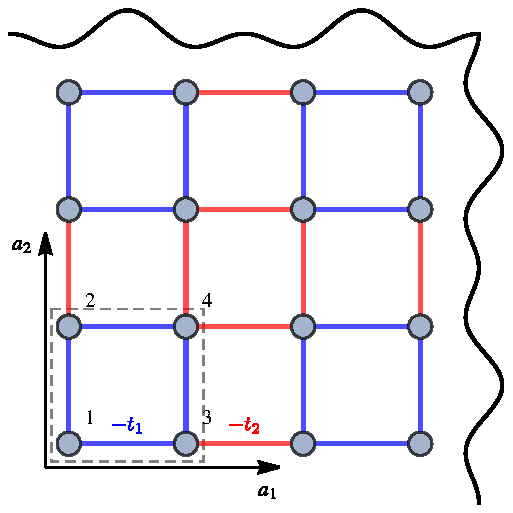
\includegraphics{FigLattice.pdf}
    \caption{\label{lattice}2D SSHBH model on a square lattice.
    A unit cell is enclosed by a gray dashed square, with four sublattices labeled by $\eta=1,\dots,4$.
    The intra-cell (inter-cell) hopping strength is $-t_1$ ($-t_2$),
    shown in blue (red) color. The real space primitive lattice vectors $a_{1,2}$ are shown as black arrows, we set $\abs{a_1}=\abs{a_2}=1$ as the length unit in this paper.}
\end{figure}
%%%%%%%%%%%%%%%%%%%%%%%%%%%%%%%%%%%%
This model Hamiltonian can be realized straightforwardly, say in 2D, by loading spinless bosons in a square optical lattice with the addition of a period-2 optical superlattice,
as illustrated in Fig.~\ref{lattice}.
Focusing on the region where $t_1 / t_2$ is not far from 1,
there is a quantum phase transition (QPT) between Mott-insulating (MI) phase and Superfluid (SF) phase driven by $t / U$,
with $t = (t_1 + t_2)/2$ \cite{Fisher1989}.
In the vicinity of this QPT at the $p$th lobe,
only three local states are relevant,
$| p + \sigma \rangle_i$,
for $\sigma = - 1, 0, 1$.
We define three commuting bosons for them,
$b_{i, \sigma}^{\dag} | 0 \rangle = | p + \sigma \rangle_i$,
with the holonomic local constraint,
$\sum_{\sigma=1}^3 b_{i, \sigma}^{\dag} b_{i, \sigma} = 1$.
Then the original boson creation operator can be written as $a^{\dag}_i = \sqrt{p + 1}
b^{\dag}_{i, + 1} b_{i, 0} + \sqrt{p} b_{i, 0}^{\dag} b_{i, - 1}$.
Up to an irrelevant constant,
and at large $p$ limit,
Eq.~(\ref{h}) becomes a pseudospin-one Hamiltonian \cite{Altman2002},
\begin{equation}
  \hat{H}_{\text{spin-1}} = \sum_{\langle i, j \rangle} \tilde{t}_{i \nocomma j}
  (\hat{S}_i^x \hat{S}_j^x + \hat{S}_i^y \hat{S}_j^y) +  \sum_i \bigg[\frac{1}{2}U
  (\hat{S}_i^z)^2 - \delta \mu \hat{S}_i^z \bigg], \label{heff}
\end{equation}
where $\langle i, j \rangle$ denotes nearest neighbors.
Here the spin operators are defined by (repeated Greek letter subscripts are summed over) $\hat{S}_i^+ = b_{i, \sigma}^{\dag} (S^+)_{\sigma \sigma'} b_{i, \sigma'}$,
$\hat{S}_i^- = (\hat{S}_i^+)^{\dag}$ and $\hat{S}_i^z = b_{i, \sigma}^{\dag} (S^z)_{\sigma \sigma'} b_{i, \sigma'}$,
with $S^z$ and $S^+$ being the spin-1 matrices in the $z$-basis.
$\delta \mu = \mu - (p - 1 / 2)U \approx \mu - pU$ is the chemical potential measured from the \emph{middle} of the $p$th lobe,
which also coincides with the \emph{tip} of the lobe when $p \gg 1$.
Thus the so-called \emph{Lorentz-invariant line} (LIL) on the $\mu / U - t / U$ phase diagram corresponds to $\delta \mu = 0$,
where there is an emergent Lorentz symmetry for the low-energy,
long-wavelength effective action \cite{Sachdev2017}.
The spin exchange interaction is given by the renormalized hopping strength, $\tilde{t}_{i \nocomma j} = pt_{i \nocomma j}$,
and we define $\tilde{t} = pt = p(t_1+t_1)/2$.
The original $\mathrm{U} (1)$ symmetry becomes the $\mathrm{O} (2)$ spin rotation symmetry along $z$ axis,
and the superfluid order parameter becomes $\psi_i = \langle a_i \rangle \approx \sqrt{p / 2} \langle \hat{S}_i^- \rangle$.

Using a Gutzwiller-type mean-field ground state ansatz $\left| \text{GS} \right\rangle = \bigotimes_i | \Phi_0 \rangle_i$,
with
\begin{eqnarray}
      | \Phi_0 \rangle_i &=& \cos \frac{1}{2}\theta \ket{0}_i + e^{i (\eta-\phi) / 2} \sin \frac{1}{2}\theta \nonumber\\
      &&  \times \left( \cos \frac{1}{2}\chi \ket{+1}_i + e^{i \phi } \sin \frac{1}{2}\chi \ket{-1}_i   \right),\nonumber
\end{eqnarray}
the ground state energy per site reads
\begin{equation}
  e_0 = \left( \frac{1}{2}U - \delta \mu \cos \chi \right) \sin^2  \frac{1}{2}\theta - \frac{1}{4} z\tilde{t} (1 + \cos \eta \sin  \chi) \sin^2 \theta , \label{mfe}
\end{equation}
where $z=2d$ is the coordination number.
Note Eq.~\eqref{mfe} is independent of $\phi$,
dictated by $\mathrm{O} (2)$ symmetry.
We set $\phi$ to be zero,
corresponding to spin polarized along $x$ direction in the SF
phase (equivalent to setting $\psi_i$ to be real).
By minimizing Eq.~(\ref{mfe}),
the ground state at the LIL (i.e., $\delta \mu = 0$) is found by setting $(\theta, \eta, \phi, \chi) = (\bar{\theta}, 0, 0, \pi / 2)$,
with $\bar{\theta} = \arccos (U / 4z \tilde{t})$ for $U < 4z \tilde{t}$,
and $\bar{\theta} = 0$ otherwise.
Via a canonical transformation,
$c_{i, \alpha}^{\dag} = b_{i, \sigma}^{\dag} T_{\sigma \alpha}$,
for $\alpha = 0, A, P$ (the nomenclature for these modes will be explained soon),
with the unitary matrix $T(\bar\theta)$ given by
\begin{equation}
   T(\bar\theta) = \begin{bmatrix}
           \frac{1}{\sqrt{2}} \sin \frac{1}{2}\bar{\theta} & \frac{- 1}{\sqrt{2}}     \cos \frac{1}{2}\bar{\theta} & \frac{1}{\sqrt{2}}\\
     \cos \frac{1}{2}\bar{\theta} & \sin \frac{1}{2}\bar{\theta} & 0\\
     \frac{1}{\sqrt{2}} \sin \frac{1}{2}\bar{\theta} & \frac{- 1}{\sqrt{2}}     \cos \frac{1}{2}\bar{\theta} & - \frac{1}{\sqrt{2}}
  \end{bmatrix},\nonumber
\end{equation}
the mean-field ground state is $\left| \text{GS} \right\rangle = \prod_i c_{i,0}^{\dag} |0 \rangle$.
To compute excitation spectra,
we condense $c_{i,0}^{(\dagger)}$ boson and treat other modes as small fluctuations.
Namely, we perform $c_{i, 0}^{(\dagger)} \rightarrow \sqrt{1 - \sum_{\alpha \neq 0} c_{i, \alpha}^{\dag} c_{i, \alpha}}$ in Eq.~(\ref{heff}) \cite{Auerbach1994},
and keep only terms up to quadratic order in operators.
The zeroth-order term gives the mean field ground state energy;
the first-order term vanishes identically;
and the second-order term can be written as two \emph{decoupled} Hamiltonians,
$\hat{H}^{(2)} = \hat{H}_{A}^{(2)} + \hat{H}_{P}^{(2)}$.
In momentum space,
these Hamiltonians can be rearranged into a Bogoliubov-de Gennes (BdG) form (subscript $\alpha$ for simplicity),
$\hat{H}^{(2)} = \frac{1}{2} \sum_{\bm{k}}\chi^{\dag}_{\bm{k}} H^{\text{BdG}}_{\bm{k}} \chi_{\bm{k}}$.
Here the Nambu spinor is defined by $\chi_{\bm{k}} = \left[\begin{array}{cc}
c_{\bm{k}} & c_{-\bm{k}}
\end{array}\right]^T$,
where $c_{\bm{k}}$ is a $2^d$-component operators,
$c_{\bm{k}, \eta}$,
with $\eta = 1, \ldots, 2^d$ labeling the sublattice.
The BdG matrix reads
\begin{equation}
  H^{\text{BdG}}_{\bm{k}} = \left[\begin{array}{cc}
    gI_{2^d\times 2^d} + \lambda M_{\bm{k}} & \mathe^{- \mathi \vartheta} \lambda M_{\bm{k}}\\
    \mathe^{\mathi \vartheta} \lambda M_{\bm{k}} & gI_{2^d\times 2^d} + \lambda M_{\bm{k}}
  \end{array}\right], \label{hbdg}
\end{equation}
where $M_{\bm{k}}$ is the Bloch Hamiltonian for the $d$D SSH model, and other parameters are given in Table.~\ref{tab:parameters}.%
%%%%%%%%%%%%%%%%%%%%%%%%%%%%%%%%%
\begin{table}[b]
\caption{\label{tab:parameters}
Parameters used in Eq.~\eqref{hbdg}, for amplitude modes ($\alpha = A$) and phase modes ($\alpha = P$). Note $\bar\theta=\arccos(U/4z\tilde t)$ for $U<4z\tilde t$, and $\bar\theta =0$ otherwise.}
\begin{ruledtabular}
\begin{tabular}{cccccccc}
 &$g$ &$\lambda$ &$\vartheta$\\
\hline
$\alpha=A$ & $2z\tilde t \sin^2\bar\theta +\frac{1}{2}U\cos\bar\theta$ & $\cos^2\bar\theta$ & $0$ \\
$\alpha=P$ & $z\tilde t\sin^2\bar\theta + \frac{1}{2}U\cos^2\frac{1}{2}\bar\theta$ & $\cos^2\frac{1}{2}\bar\theta$ & $\pi$
\end{tabular}
\end{ruledtabular}
\end{table}
%%%%%%%%%%%%%%%%%%%%%%%%%%%%%%%%%
The Bogoliubov transformation that diagonalizes Eq.~(\ref{hbdg}) can be constructed analytically from the noninteracting Hamiltonian $M_{\bm{k}}$ \cite{Kumar2020}.
Namely,
assuming that the unitary matrix $Q_{\bm{k}}$ diagonalizes $M_{\bm{k}}$,
$Q_{\bm{k}}^{\dag} M_{\bm{k}} Q_{\bm{k}} = \text{diag} \{m_{1, \bm{k}}, \ldots, m_{2^d, \bm{k}} \}$,
we define two hyperbolic functions $\cosh\beta_{i, \bm{k}} = \sqrt{\frac{g + m_{i, \bm{k}}}{2 E_{i,\bm{k}}} + \frac{1}{2}}$,
$\sinh \beta_{i, \bm{k}} = - \tmop{sign}(m_{i, \bm{k}}) \sqrt{\frac{g_{\alpha} + m_{i, \bm{k}}}{2 E_{i,\bm{k}}} - \frac{1}{2}}$,
with
\begin{equation}
  E_{i, \bm{k}} = \sqrt{g^2 + 2 g m_{i, \bm{k}}}, \label{eb}
\end{equation}
and two associated diagonal matrices $C_{\bm{k}} = \text{diag} \{ \cosh \beta_{1, \bm{k}}, \ldots, \cosh \beta_{2^d,\bm{k}} \}$,
and $S_{\alpha, \bm{k}} = \text{diag} \{ \sinh \beta_{1,\bm{k}}, \ldots, \sinh \beta_{2^d, \bm{k}} \}$.
Then the needed pseudounitary transformation is
\begin{equation}
  W_{\bm{k}}^{\dag} (\Sigma_z H^\tbdg_{\vb k}) W_{\bm{k}}  = \tau_z \otimes \begin{bmatrix}
      E_{1, \bm{k}} & & \\
      & \ddots & \\
      & & E_{2^d,\bm{k}}
  \end{bmatrix},\label{put}
\end{equation}
where $\Sigma_z=\tau_z\otimes I_{2^d}$. And the pseudounitary matrix explicitly reads $W_{\bm{k}} = \tilde Q_{\bm{k}} P_{\bm{k}}$,
where $\tilde Q_{\bm{k}}=\tau_0 \otimes Q_{\bm{k}}$,
and $P_{\bm{k}} = \tau_0 \otimes C_{\bm{k}} + \tau_1 \otimes S_{\bm{k}}$,
with $\tau_i$,
for $i=1,2,3$ and $i=0$,
being the three Pauli matrices,
and two-by-two identity matrix,
respectively, acting on the Nambu space.

%%%%%%%%%%%%%%%%%%%%%%%%%%%%%%%%%%%%%%%
\begin{figure}[t]
    \includegraphics{FigSpin1OBC.pdf}
    \caption{\label{spin1OBC} Excitation spectrum of the 2D SSHBH model on a ribbon geometry.
    (a) ($t_1/t_2=3$) and (b) ($t_2/t_1=3$) corresponds to the Higgs amplitude modes.
    (c) ($t_1/t_2=3$) and (d) ($t_2/t_1=3$) corresponds to the phase modes.
    Two blue curves,
    which are doubly degenerated due to inversion symmetry,
    are topological edge states whose wave functions have more than $66\%$ weight on the edge unit cells.
    Other parameters:
    $U=0.95 U_c$ with $U_c=4z \tilde t$ corresponding to the phase transition point.}
\end{figure}
%%%%%%%%%%%%%%%%%%%%%%%%%%%%%%%%%%%%%%%

For a given low-energy excitation labeled by momentum $\bm{k}$ and band index $\lambda$,
it produces a perturbation with respect to the ground state expectation value for a given operator $O_i$ as $\delta O_i = \expval{O_i}_{\bm k,\lambda}-\expval{O_i}_0$.
Up to linear order in fluctuations,
the oscillation induced by two types of modes $\alpha = A$ and $P$,
for the spin operator $\hat{\bm{S}}_i$,
is given by
\begin{subequations}\label{per}
    \begin{align}
        \delta \bm{S}_i^{(A)} &= f^{(A)}_{\bm{k}, \lambda} \cos (E_{i, \alpha,
  \bm{k}} t -\bm{k} \cdot \bm{r}) \hat{\bm{e}}_x,
  \label{dsa}\\
   \delta \bm{S}_i^{(P)} &= f^{(P)}_{ \bm{k}, \lambda} \sin (E_{k,
  \lambda} t -\bm{k} \cdot \bm{r}_i) \hat{\bm{e}}_y \nonumber\\
 &\quad + f^{(P)\prime}_{\bm{k}, \lambda} \cos (E_{k, \lambda} t -\bm{k} \cdot
  \bm{r}_i) \hat{\bm{e}}_z, \label{dsp}
    \end{align}
\end{subequations}
where three coefficients $f^{(A)}_{\bm{k}, \lambda} = - [Q_{\bm{k}}]_{\eta \lambda} g^{(A)}_{\lambda, \bm{k}} \cos \bar{\theta}$,
$f^{(P)}_{\bm{k}, \lambda}= - [Q_{\bm{k}}]_{\eta \lambda} g^{(P)}_{\lambda, \bm{k}} \cos\frac{1}{2}\bar{\theta}$,
and $f^{(P)\prime}_{\bm{k}, \lambda} = -[Q_{\bm{k}}]_{\eta \lambda} g^{(P)}_{\lambda, \bm{k}} \sin\frac{1}{2}\bar{\theta}$, with $g^{(\alpha)}_{\lambda, \bm{k}} = \sinh\beta^{(\alpha)}_{\lambda, \bm{k}} + \cosh \beta^{(\alpha)}_{\lambda,
\bm{k}}$, are real numbers if a suitable gauge of $Q_{\bm{k}}$ is chosen.
Eq.~\eqref{dsa} therefore identifies $A$ modes as the Higgs amplitude modes since they induce longitudinal oscillation of spins;
while Eq.~\eqref{dsp} identifies $P$ modes as the phase modes (i.e., magnon) since they induce transverse oscillation of spins (i.e., precession).
Additionally, noticing that
\begin{equation}
  \delta\psi_i = (\rho_0 + \delta \rho_i) \mathe^{\mathi \delta \phi_i} - \rho_0
  \approx \delta \rho_i + \mathi \rho_0 \delta \phi_i, \label{op}
\end{equation}
the pure amplitude $\rho$ and phase $\phi$ oscillation correspond to $\delta \psi_i$ with vanishing imaginary and real part, respectively.
This is equivalent to the absence of spin fluctuations in $y$ and $x$ direction, since $a_i \propto S_i^- = S_i^x - \mathi S_i^y$.
Eq.~\eqref{per} therefore again comfirms the existence of the pure Higgs amplitude bands in the large $p$ limit, within the original boson language,.

We now show that the Higgs amplitude bands inherit topological character of the underlying $d$D SSH model.
Recall that the latter is known as a topological crystalline insulator protected by inversion symmetry,
\begin{equation}
  \mathcal{I}M_{\bm{k}} \mathcal{I}^{- 1}  =M_{-\bm{k}}, \label{is0}
\end{equation}
with the associated topological invariant being the vectorized Zak phase,
also equal to the macroscopic polarization vector,
defined by \cite{Liu2017}
\begin{equation}
  \bm{P}= \frac{1}{2 \pi} \int \mathd^2 k \tmop{Tr} [\bm{A}
  (\bm{k})], \label{mpv}
\end{equation}
where the Berry connection reads $A_i = \mathi \sum_{\lambda\leq\lambda_{\text{max}}} \tmop{Tr} [\Gamma_\lambda Q^{\dag}_{\bm{k}} \partial_{k_i} Q_{\bm{k}}]$,
for $i=x_1,\dots,x_d$,
and $\Gamma_\lambda$ is a $2^d$-by-$2^d$ matrix with $\lambda$th diagonal component being $+ 1$ and all others vanishing.
$\lambda_{\text{max}}$ is the maximal band index of the occupied bands.
The integration is taken over the first Brillouin zone (1BZ).
Due to inversion symmetry,
each component of $\bm{P}$ is restrictedly quantized as a $\mathbb{Z}_2$ index \cite{Fang2012},
\begin{equation}
  P_i = \frac{i}{2 \pi} \ln \left[ \prod_{\lambda\leq\lambda_{\text{max}}} \eta_{\lambda} (\Gamma)
  \eta_{\lambda} (X_i) \right], \label{p}
\end{equation}
where $\eta_{\lambda}$ is the eigenvalue of the inversion operator $\mathcal I$ for the $\lambda$th band,
and $X_i$ is the inversion symmetric momentum other than $\Gamma$ on the $x_i$ axis in the 1BZ.
The band inversion points occur at all $X_i$'s when $t_1 = t_2$, as a consequence of, say in 2D, the $\mathrm{C}_{4v}$ symmetry.
For $t_1 < t_2$,
the system is in the topological phase,
with $\bm{P}= \left(1/2,\dots, 1/2 \right)$;
otherwise the system is in the trivial phase with $\bm{P}= (0,\dots, 0)$.
Returning to the bosonic BdG system defined by Eq.~(\ref{hbdg}),
the single-particle inversion symmetry operator is promoted by extending it to the Nambu space as $\mathcal{I}_{\tau} = \tau_0 \otimes \mathcal{I}$,
and the inversion symmetry is defined by
\begin{equation}
  \mathcal{I}_{\tau} H^{\text{BdG}}_{\bm{k}} \mathcal{I}_{\tau}^{- 1} = H^{\text{BdG}}_{-\bm{k}},\label{is}
\end{equation}
with the associated topological invariant also given by Eq.~(\ref{mpv}),
where the bosonic Berry connection being $A_i = \mathi \sum_{\lambda\leq\lambda_{\text{max}}} \tmop{Tr} [\Gamma_\lambda \Sigma_3 W_{\bm{k}}^{\dag} \Sigma_3 \partial_{k_i} W_{\bm{k}}]$ \cite{Shindou2013}.
The quantity $\bm{P}$ defined in this way is called the vectorized symplectic polarization,
which is again quantized due to inversion symmetry \cite{Engelhardt2015},
described also by Eq.~\eqref{p}.
Using $W_{\bm{k}}$ defined in Eq.~\eqref{put},
it can be shown straightforwardly that
\begin{equation}
  W_{\bm{K}}^{\dag} \Sigma_z \mathcal{I}_\tau W_{\bm{K}} = \tau_z
  \otimes \begin{bmatrix}
      \eta_{1,\bm{K}} & &\\
      & \ddots & \\
      & & \eta_{2^d,\bm{K}}
  \end{bmatrix} ,\nonumber
\end{equation}
where $\bm{K}$ is an inversion symmetric momentum.
Thus the parities of the BdG system is the same as the $d$D SSH model.
Moreover,
Eq.~\eqref{eb} indicates that the spectra of the BdG system is a smooth and monotonically increasing function of the $d$D SSH model's.
It follows that the transition between topological ($t_1 < t_2$) and trivial ($t_1 > t_2$) excitation spectra also happens at $t_1 = t_2$.

According to the bulk-boundary correspondence (BBC),
non-trivial bulk topology implies the existence of topological edge modes for systems under open boundary conditions (OBCs).
Here we numerically verify the BBC for the Higgs amplitude modes and the phase modes by considering a ribbon geometry.
As shown in Fig.~\ref{spin1OBC},
the presence or absence of topological edge modes indeed goes hand in hand with the bulk quantized index.

%%%%%%%%%%%%%%%%%%%%%%%%%%%%%%%%%%%%%%%
\begin{figure*}
    \includegraphics{FigSBPBCOBC.pdf}
    \caption{\label{pbcobc}Excitation spectrum of the 2D SSHBH model under (a) PBCs  and (b) on a ribbon geometry,
    with the colored indicating the flatness defined in Eq.~\eqref{flatness}.
    The filling factor $p=2$ for (a1) and (b1),
    $p=30$ for (a2) and (b2),
    and $p=120$ for (a3) and (b3).
    Points representing the topological edge modes are plotted in larger size in (b).
    Other parameters:
    $U=0.95 U_c$, $t_2/t_1=3$, and the chemical potential $\mu$ is chosen to make the system on the LIL.}
\end{figure*}
%%%%%%%%%%%%%%%%%%%%%%%%%%%%%%%%%%%%%%%
